% Asal-usul (tidak pernah dicetak): lihat sources/outline_sources.md (Tahun 1: hotspot dan
% plume mantel; rantai hotspot dan gerak absolut lempeng; provinsi beku besar). Peta hotspot,
% pencocokan kutub, laju dan tonjolan dari figdata/bachelor-1/hotspots.py (data
% data/derived/bachelor-1-hotspots.csv, Tabel 1 suplemen elektronik Morgan dan Morgan 2007);
% nilai soal latihan dan soal dihitung dalam kalkulator skrap Buku 3 calc/ch15.py dan
% calc/ch15ex.py. "Hotspot" dibangun ulang dari Buku 1 (gunung api kelas 7), "jejak hotspot"
% dari Buku 2 (gerak lempeng kelas 11); Buku 2 memiliki kecocokan jarak--umur rantai Hawaii,
% sehingga bab ini mencocokkan kutub Euler Pasifik dari arah jejak sebagai gantinya.
\chapter{Hotspot dan vulkanisme intralempeng}\label{ch:b1:hotspots}

Dari Januari 1983, dan selama puluhan tahun sesudahnya, Kilauea, di pulau Hawaii, meletus hampir tanpa jeda dari kawah di zona celah timurnya, Pu\textquoteleft u~\textquoteleft O\textquoteleft o, mengalirkan sekitar \qty{0.12}{km^3} lava setahun. Kilauea berdiri di tengah Lempeng Pasifik, ribuan kilometer dari punggungan atau palung mana pun. Ke barat laut, pulau-pulau Hawaii semakin tua, lalu tenggelam di bawah laut dan rantainya berlanjut sebagai deretan gunung api yang tenggelam sejauh ribuan kilometer lagi. Tektonik lempeng menjelaskan gunung api di batas lempeng; bab ini membahas yang tidak langsung dijelaskannya, yaitu \omterm{def:b1:hotspots:hotspot}{hotspot}, dan apa yang mereka ungkapkan sebagai balasan: bagaimana lempeng bergerak di atas \omterm{def:b1:layered-earth:layers}{mantel} dalam, berapa banyak panas dan batuan naik dari bawah, dan bagaimana beberapa luapan lava yang sangat besar, \omterm{def:b1:hotspots:lip}{provinsi beku besar}, terbentuk.
% ledger: pp1801:kilauea-rate

\begin{recall}
\omterm{def:b1:hotspots:hotspot}{Hotspot} memberi makan gunung api dari jauh di dalam \omterm{def:b1:layered-earth:layers}{mantel} sementara lempeng bergerak di atasnya, dan lempeng membawa pergi \omterm{def:b1:hotspots:track}{jejak hotspot} yang gunung apinya semakin tua dengan jarak (Buku 1, kelas 7; Buku 2, kelas 11). Lempeng yang berputar dengan \omterm{def:b1:plate-kinematics:euler-pole}{vektor Euler} $\vec\omega$ bergerak dengan $\vec v = \vec\omega\times\vec r$, dengan laju $\omega R\sin\Delta$, tegak lurus terhadap \omterm{def:b1:spherical-astronomy:spherical-triangle}{lingkaran besar} yang menghubungkannya dengan kutub (\cref{ch:b1:plate-kinematics}); relief ditopang oleh \omterm{def:b1:isostasy-gravity:isostasy}{isostasi} (\cref{ch:b1:isostasy-gravity}); batuan yang hangat lebih ringan sebesar pecahan $\alpha\,\Delta T$ (\cref{ch:b1:rifts-ridges-margins}).
\end{recall}

\section{Hotspot dan plume mantel}\label{sec:b1:hotspots:plumes}

\begin{definition}[Hotspot (titik panas)]\label{def:b1:hotspots:hotspot}
Sebuah \emph{hotspot}\index{hotspot} adalah wilayah vulkanisme yang posisinya tidak bergantung pada batas lempeng, aktif selama puluhan juta tahun, dan diperkirakan diberi makan oleh \omterm{def:b1:layered-earth:layers}{mantel} yang lebih panas daripada \omterm{def:b1:layered-earth:layers}{mantel} di sekitarnya.
\end{definition}

Berapa banyak \omterm{def:b1:hotspots:hotspot}{hotspot} yang ada bergantung pada apa yang dihitung. Tabel \omterm{def:b1:hotspots:hotspot}{hotspot} yang dipakai dalam bab ini mendaftar 68 di antaranya, tetapi penulisnya meninggalkan beberapa kenampakan yang mereka nilai tidak mencatat gerak suatu lempeng, dan mereka menilai sebagian yang mereka simpan hanya sebagai kemungkinan. Beberapa \omterm{def:b1:hotspots:hotspot}{hotspot}, di antaranya Hawaii, Islandia dan Réunion, memiliki jejak yang panjang dan teratur serta keluaran yang besar, seperti yang diharapkan dari sumber dalam; yang lain kecil dan berumur pendek. Sebagian besar gunung api \omterm{def:b1:hotspots:hotspot}{hotspot} mengeluarkan basal; ketika \omterm{def:b1:hotspots:hotspot}{hotspot} berada di bawah benua, basal panas melelehkan \omterm{def:b1:layered-earth:layers}{kerak}, dan letusan besar berubah menjadi riolit, seperti di Yellowstone.
% ledger: mm07:table, data:b3-hotspots, yvo:calderas

\begin{definition}[Plume mantel]\label{def:b1:hotspots:plume}
Sebuah \emph{plume mantel}\index{plume mantel} adalah kolom batuan \omterm{def:b1:layered-earth:layers}{mantel} yang panas dan apung, yang naik dari \omterm{def:b1:heat-budget:boundary-layer}{lapisan batas termal} yang dalam di \omterm{def:b1:layered-earth:layers}{mantel}. Plume baru memiliki \emph{kepala} besar berbentuk umbi di atas \emph{ekor}, atau saluran, yang panjang dan sempit; setelah kepala itu menyebar di bawah \omterm{def:b1:layered-earth:lithosphere}{litosfer}, ekornya terus mengalirkan lelehan ke permukaan selama puluhan juta tahun.
\end{definition}

Bentuknya berasal dari laboratorium. Dalam eksperimen tangki pada 1970-an, lapisan fluida ringan yang lebih encer daripada fluida di atasnya naik sebagai kantong bulat yang diumpankan oleh pipa di belakangnya: sebuah jamur. Kepala \omterm{def:b1:hotspots:plume}{plume mantel} yang mencapai dasar \omterm{def:b1:layered-earth:lithosphere}{litosfer} menyebar dan mendatar; tekanannya turun, dan batuan panas meleleh dalam jumlah besar. Basal banjir sesuai dengan gambaran ini: vulkanismenya berlangsung sekitar sepuluh juta tahun, tetapi sebagian besar volumenya meletus dalam sekitar satu juta tahun atau kurang, dan sering kali berjalan seiring dengan pecahnya benua (\cref{sec:b1:hotspots:lips}).
% ledger: hist:plumes (Whitehead and Luther 1975), cr03:summary

\begin{omfigure}
\begin{tikzpicture}[font=\scriptsize,
  lbl/.style={fill=white, fill opacity=0.8, text opacity=1, inner sep=1pt, align=center}]
% ---- panel (a): the head arrives ----
\begin{scope}
\clip (0,-5) rectangle (6.4,1.3);
\fill[orange!12] (0,-5) rectangle (6.4,0);
\fill[omSea!45] (0,0) rectangle (6.4,0.55);
\fill[omLithBasalt!55] (0,0) rectangle (6.4,-0.9);
% flood basalt: a stack of flat flows on the sea floor
\fill[black!55] (2.5,0) -- (2.7,0.32) -- (6.1,0.32) -- (6.3,0) -- cycle;
\foreach \y in {0.08,0.16,0.24} \draw[white!70!black, line width=0.3pt] (2.62,\y) -- (6.18,\y);
% plume: tail and flattened head
\fill[red!40] (4.25,-5) -- (4.25,-1.7) -- (4.55,-1.7) -- (4.55,-5) -- cycle;
\fill[red!40] (4.4,-1.45) ellipse[x radius=1.9, y radius=0.55];
\draw[red!60!black, line width=0.4pt] (4.25,-5) -- (4.25,-1.95) (4.55,-5) -- (4.55,-1.95);
\draw[red!60!black, line width=0.4pt] (4.4,-1.45) ellipse[x radius=1.9, y radius=0.55];
% melt rising through the plate
\foreach \x in {3.2,3.9,4.6,5.3}
  \draw[red!75!black, line width=0.6pt, decorate, decoration={snake, amplitude=0.6pt, segment length=3pt}] (\x,-1.1) -- (\x,0.05);
\end{scope}
\draw[black!70] (0,-5) rectangle (6.4,1.3);
\node[lbl, anchor=north west] at (0.1,1.25) {(a) kepala tiba};
\node[lbl, anchor=west] at (0.1,-0.45) {litosfer};
\node[lbl, anchor=west] at (0.1,0.3) {laut};
\node[lbl, anchor=south] at (4.4,0.62) {basal banjir (provinsi beku)};
\node[lbl, anchor=east] (ph) at (1.9,-1.75) {kepala plume};
\draw[black!70] (ph.east) -- (2.7,-1.6);
\node[lbl, anchor=east] at (4.1,-3.6) {ekor plume};
\node[lbl, anchor=west] at (0.1,-4.6) {mantel};
% ---- panel (b): the plate has moved on ----
\begin{scope}[xshift=6.8cm]
\begin{scope}
\clip (0,-5) rectangle (6.4,1.3);
\fill[orange!12] (0,-5) rectangle (6.4,0);
\fill[omSea!45] (0,0) rectangle (6.4,0.55);
\fill[omLithBasalt!55] (0,0) rectangle (6.4,-0.9);
% the flood basalt, carried away to the left
\fill[black!55] (-0.9,0) -- (-0.7,0.32) -- (1.0,0.32) -- (1.2,0) -- cycle;
\foreach \y in {0.08,0.16,0.24} \draw[white!70!black, line width=0.3pt] (-0.8,\y) -- (1.08,\y);
% the chain: older volcanoes to the left, lower (they sank as the plate cooled)
\fill[black!35] (1.45,0) -- (1.75,0.2) -- (2.05,0) -- cycle;
\fill[black!38] (2.15,0) -- (2.5,0.3) -- (2.85,0) -- cycle;
\fill[black!42] (2.95,0) -- (3.35,0.42) -- (3.75,0) -- cycle;
\fill[black!65] (3.95,0) -- (4.45,0.95) -- (4.55,0.97) -- (5.05,0) -- cycle;
\fill[red!70!black] (4.43,0.93) -- (4.57,0.95) -- (4.5,1.12) -- cycle;
% the plume tail, still in place, and a small spread of hot rock under the plate
\fill[red!40] (4.35,-5) -- (4.35,-1.1) -- (4.65,-1.1) -- (4.65,-5) -- cycle;
\fill[red!40] (4.5,-1.05) ellipse[x radius=0.75, y radius=0.2];
\draw[red!60!black, line width=0.4pt] (4.35,-5) -- (4.35,-1.2) (4.65,-5) -- (4.65,-1.2);
\draw[red!75!black, line width=0.6pt, decorate, decoration={snake, amplitude=0.6pt, segment length=3pt}] (4.5,-0.95) -- (4.5,0.8);
\end{scope}
\draw[black!70] (0,-5) rectangle (6.4,1.3);
\node[lbl, anchor=north west] at (0.1,1.25) {(b) jauh kemudian};
\draw[->, line width=1pt] (3.2,-0.45) -- (1.2,-0.45) node[midway, above=1pt, lbl] {gerak lempeng};
\node[lbl, anchor=south] at (0.55,0.38) {provinsi beku};
\node[lbl, anchor=south] at (2.7,0.62) {lebih tua, punah};
\node[lbl, anchor=west] at (5.0,0.95) {gunung api\\aktif};
\node[lbl, anchor=east] at (4.2,-3.6) {ekor plume};
\node[lbl, anchor=west] at (4.75,-2.6) {tetap di\\dalam mantel};
\end{scope}
\end{tikzpicture}
\par\smallskip{\small Model plume sebuah \omterm{def:b1:hotspots:hotspot}{hotspot} (skematik, tidak sesuai skala). (a)~Plume baru: kepalanya mendatar di bawah \omterm{def:b1:layered-earth:lithosphere}{litosfer} dan meleleh ketika tekanannya berkurang, dan basal banjir, \omterm{def:b1:hotspots:lip}{provinsi beku besar}, meletus dalam beberapa juta tahun atau kurang. (b)~Puluhan juta tahun kemudian lempeng telah membawa provinsi itu pergi; ekor yang sempit masih memberi makan gunung api yang aktif, dan gunung api yang dibangunnya sebelumnya telah punah, lebih tua dengan jarak, dan lebih rendah, karena mereka tenggelam bersama lempeng yang mendingin.}
\label{fig:b1:hotspots:plume}
\end{omfigure}

Apa buktinya untuk plume? Pertama, rantai yang umurnya progresif itu sendiri, yang dijelaskan sekaligus oleh sumber sempit yang tetap di bawah lempeng yang bergerak (\cref{sec:b1:hotspots:tracks}). Kedua, lava beberapa \omterm{def:b1:hotspots:hotspot}{hotspot} membawa rasio yang luar biasa tinggi antara isotop helium yang ringan dan yang berat, yang dibaca sebagai tanda reservoir dalam yang telah menyimpan sebagian gas yang dengannya Bumi dibentuk. Ketiga, sumbernya panas: lava pulau samudra dan dataran tinggi menunjuk ke \omterm{def:b1:layered-earth:layers}{mantel} 200 hingga \qty{300}{\celsius} lebih panas daripada \omterm{def:b1:layered-earth:layers}{mantel} di bawah punggungan, yang suhu potensialnya berada antara 1280 dan \qty{1400}{\celsius}. Keempat, citra seismik \omterm{def:b1:layered-earth:layers}{mantel}: di bawah Hawaii, jaringan seismometer di dasar laut dan di pulau-pulau mencitrakan kolom panas yang menjulur ke \omterm{def:b1:layered-earth:layers}{mantel} bawah, dan model seluruh \omterm{def:b1:layered-earth:layers}{mantel} yang dibangun pada 2015 dari bentuk gelombang seismik lengkap memperlihatkan kolom lebar yang kurang lebih vertikal di bawah banyak \omterm{def:b1:hotspots:hotspot}{hotspot} utama, naik dari \omterm{def:b1:layered-earth:discontinuity}{batas inti--mantel} hingga sekitar \qty{1000}{km} di bawah permukaan; di bawah Hawaii, Islandia dan Samoa mereka berakar pada bidang-bidang berkecepatan gelombang sangat rendah di dasar \omterm{def:b1:layered-earth:layers}{mantel}. Bagaimana citra semacam itu dibuat termasuk dalam volume Tahun ke-3.
% ledger: herzberg:tp, wolfe:hawaii, fr15:plumes

Ini belum merupakan bukti, dan perdebatannya masih hidup. Dalam hipotesis lempeng, yang dibela antara lain oleh Gillian Foulger dan James Natland, vulkanisme \omterm{def:b1:hotspots:hotspot}{hotspot} tidak terutama panas dan tidak memerlukan plume dalam: ia adalah produk sampingan tektonik lempeng, diberi makan dari sumber dangkal tempat \omterm{def:b1:layered-earth:lithosphere}{litosfer} teregang atau retak. Para penentangnya berpendapat bahwa bukti bagi sekurang-kurangnya sebagian plume dalam kuat, meskipun citra seismiknya belum cukup tajam untuk memutuskannya; dan \omterm{def:b1:hotspots:hotspot}{hotspot}, seperti yang ditunjukkan bagian berikutnya, tidak sepenuhnya tetap.
% ledger: fn03:plate-hypothesis, tarduno:emperor

\section{Jejak hotspot dan gerak lempeng}\label{sec:b1:hotspots:tracks}

\begin{definition}[Jejak hotspot; progresi umur]\label{def:b1:hotspots:track}
Sebuah \emph{jejak hotspot}\index{jejak hotspot} adalah deretan gunung api, gunung laut dan punggungan vulkanik yang dibawa menjauh oleh lempeng dari \omterm{def:b1:hotspots:hotspot}{hotspot} saat ia bergerak di atasnya. \emph{Progresi umur}\index{progresi umur} adalah peningkatan teratur umur gunung-gunungnya terhadap jarak dari yang aktif. \emph{Arah} sebuah jejak di \omterm{def:b1:hotspots:hotspot}{hotspot} adalah \omterm{def:b1:spherical-astronomy:horizontal}{azimut}, diukur dari utara, ke arah bagian mudanya menjauh dari \omterm{def:b1:hotspots:hotspot}{hotspot}.
\end{definition}

Jika \omterm{def:b1:hotspots:hotspot}{hotspot} tetap di \omterm{def:b1:layered-earth:layers}{mantel} dalam, sebuah jejak mencatat gerak lempeng di atas \omterm{def:b1:layered-earth:layers}{mantel} dalam: arahnya adalah arah kecepatan lempeng di \omterm{def:b1:hotspots:hotspot}{hotspot}, dan \omterm{def:b1:hotspots:track}{progresi umurnya} memberi lajunya. Buku 2, kelas 11, membaca laju Lempeng Pasifik dari umur gunung-gunung api Hawaii. Arahnya saja sudah mengatakan lebih banyak: arah itu memberi \omterm{def:b1:plate-kinematics:euler-pole}{kutub Euler}.

\begin{proposition}[Kutub Euler dari dua jejak]\label{prop:b1:hotspots:two-tracks}
Anggaplah sebuah \omterm{def:b1:plate-kinematics:rigid-plate}{lempeng kaku} bergerak di atas dua \omterm{def:b1:hotspots:hotspot}{hotspot} tetap pada posisi $\vec r_1$ dan
$\vec r_2$, dan biarkan $\vec t_1$ dan $\vec t_2$ menjadi vektor satuan horizontal sepanjang
jejak-jejaknya. Jika $\vec t_1$ dan $\vec t_2$ tidak sejajar, \omterm{def:b1:plate-kinematics:euler-pole}{vektor Euler} lempeng relatif
terhadap \omterm{def:b1:hotspots:hotspot}{hotspot} sejajar dengan $\vec t_1\times\vec t_2$, dan kutubnya adalah vektor satuan
\[
  \vec p = \pm\frac{\vec t_1\times\vec t_2}{\lVert\vec t_1\times\vec t_2\rVert},
\]
dengan tanda yang untuknya $(\vec p\times\vec r_1)\cdot\vec t_1 > 0$.
\end{proposition}

\begin{proof}
Di setiap \omterm{def:b1:hotspots:hotspot}{hotspot} lempeng bergerak dengan $\vec v_i = \vec\omega\times\vec r_i$
(\cref{thm:b1:plate-kinematics:velocity}), dan jejak itu mengikutinya:
$\vec v_i = v_i\vec t_i$ dengan $v_i > 0$. Hasil kali silang tegak lurus terhadap faktor-faktornya,
sehingga $\vec\omega\cdot\vec t_i = 0$ untuk $i = 1, 2$: $\vec\omega$ tegak lurus terhadap dua
vektor yang tidak sejajar, sehingga sejajar dengan hasil kali silangnya. Dari dua vektor
satuan sepanjangnya, kutubnya adalah yang rotasinya berlawanan arah jarum jam, yaitu yang
untuknya $\vec p\times\vec r_1$ menunjuk ke arah lempeng bergerak di \omterm{def:b1:hotspots:hotspot}{hotspot} pertama,
sepanjang $+\vec t_1$.
\end{proof}

Untuk menggunakan proposisi, di sebuah titik pada \omterm{def:b1:spherical-astronomy:geographic}{lintang} $\varphi$ dan \omterm{def:b1:spherical-astronomy:geographic}{bujur} $\lambda$
diperlukan vektor satuan yang menunjuk ke timur dan ke utara,
\[
  \vec e = (-\sin\lambda,\ \cos\lambda,\ 0),\qquad
  \vec n = (-\sin\varphi\cos\lambda,\ -\sin\varphi\sin\lambda,\ \cos\varphi),
\]
dalam sumbu \cref{ch:b1:plate-kinematics} ($x$ ke arah \ang{0}\,LU \ang{0}\,BT, $y$ ke arah
\ang{0}\,LU \ang{90}\,BT, $z$ ke arah kutub utara). Jejak dengan \omterm{def:b1:spherical-astronomy:horizontal}{azimut} $\theta$ berjalan
sepanjang $\vec t = \sin\theta\,\vec e +
\cos\theta\,\vec n$. Dengan jejak Hawaii, \omterm{def:b1:spherical-astronomy:horizontal}{azimut} \ang{304}, dan jejak Louisville, \omterm{def:b1:spherical-astronomy:horizontal}{azimut} \ang{316},
proposisi menempatkan kutub Lempeng Pasifik pada \ang{56.2}\,LS, \ang{124.0}\,BT (soal akhir
pekan melakukan perhitungan itu).
% values (hotspots.py): two_pole_lat -56.1805, two_pole_lon 124.008; ledger: data:b3-hotspots

Dua jejak menentukan kutub tetapi tidak dapat mengujinya. Banyak jejak melebihi-tentukan,
dan simpangannya memberitahu apakah \omterm{def:b1:hotspots:hotspot}{hotspot} berperilaku sebagai kerangka tetap. W. Jason
Morgan, yang mengusulkan plume dalam, dan Jason Phipps Morgan menyusun pada 2007 sebuah
tabel berisi 68 \omterm{def:b1:hotspots:hotspot}{hotspot}, dengan, di tempat yang dapat diukur, arah jejak dan laju lempeng
di atas \omterm{def:b1:hotspots:hotspot}{hotspot}, masing-masing dengan ketidakpastiannya dan bobot untuk keandalannya;
\omterm{def:b1:hotspots:hotspot}{hotspot} di bawah dua lempeng, seperti Islandia, memiliki satu baris untuk masing-masing.
Lima belas jejak berbobot terletak di Lempeng Pasifik, tiga belas di antaranya dengan laju.
% ledger: data:b3-hotspots, mm07:table; values (hotspots.py): n_all 71 rows, n_pacific 15, n_rated 13

\begin{method}[Mencocokkan kutub Euler dan laju pada jejak hotspot]\label{met:b1:hotspots:pole-fit}
Diberikan, untuk $N$ \omterm{def:b1:hotspots:hotspot}{hotspot} pada satu lempeng, posisinya, arah jejak
$\theta_i \pm \sigma_i$ dengan bobot $w_i$, dan untuk sebagian di antaranya lajunya
$v_i$:
\begin{enumerate}
  \item Untuk kutub percobaan $\vec p$, hitung di setiap \omterm{def:b1:hotspots:hotspot}{hotspot} arah $\vec p\times\vec r_i$,
        \omterm{def:b1:spherical-astronomy:horizontal}{azimut} $\hat\theta_i$ dari gerak yang diprediksinya
        (\cref{prop:b1:plate-kinematics:speed}).
  \item Bentuk simpangan $S(\vec p) = \sum_i w_i\bigl((\hat\theta_i -
        \theta_i)/\sigma_i\bigr)^2$, dengan setiap selisih dibawa ke antara
        \ang{-180} dan \ang{180}.
  \item Cari kutub yang meminimumkan $S$: pada kisi seluruh bola, lalu pada kisi yang lebih
        halus di sekitar titik terbaik.
  \item Dengan kutub yang ditemukan, hitung untuk setiap \omterm{def:b1:hotspots:hotspot}{hotspot} yang punya laju jarak sudutnya
        $\Delta_i$ ke kutub dan $x_i = R\sin\Delta_i$. Lajunya seharusnya $v_i = \omega x_i$:
        laju kuadrat terkecilnya adalah
        \[
          \omega = \frac{\sum_i x_i v_i}{\sum_i x_i^2},
        \]
        karena $\frac{\mathrm d}{\mathrm d\omega}\sum_i (v_i - \omega x_i)^2 =
        -2\sum_i x_i(v_i - \omega x_i)$ lenyap di sana.
  \item Nilai kecocokannya: jika \omterm{def:b1:hotspots:hotspot}{hotspot} tetap dan ketidakpastiannya jujur, $S$ akan dekat dengan
        jumlah arah dikurangi dua (dua koordinat kutub yang dicocokkan).
\end{enumerate}
\end{method}

Untuk lima belas jejak Pasifik, metode ini memberi kutub \ang{63.8}\,LS,
\ang{112.5}\,BT, sekitar \ang{10} dari kutub dua jejak, dan dari tiga belas laju itu memberi
$\omega = \qty{0.92}{\degree\per\Ma}$. Di Hawaii, \ang{108.0} dari kutub, kecocokan
memprediksi gerak ke arah \ang{298} sebesar \qty{97}{mm.yr^{-1}}; Morgan dan Morgan mencantumkan
$\ang{304}\pm\ang{3}$ dan \qty[uncertainty-mode=separate]{92 \pm 3}{mm.yr^{-1}}. Simpangan $S$
adalah 39, sedangkan \omterm{def:b1:hotspots:hotspot}{hotspot} tetap dengan ketidakpastian jujur akan memberi sekitar 13, dan lajunya
tersebar di sekitar garis sebesar \qty{16}{mm.yr^{-1}} (akar rata-rata kuadrat): \omterm{def:b1:hotspots:hotspot}{hotspot} Pasifik
membentuk kerangka acuan yang baik hingga beberapa derajat dan beberapa sentimeter setahun,
tidak lebih baik.
% values (hotspots.py): pole_lon 112.48, pole_lat -63.78, chi2 38.7829, omega_deg_myr 0.920609,
% hawaii_delta 107.998, hawaii_pred_az 297.656, hawaii_pred_rate 97.3581, rms_rate 15.966;
% angle between the two poles 9.5 deg (calc/ch15.py); ledger: data:b3-hotspots

Tes terbaik untuk kerangka tetap adalah lengkungan rantai Hawaii--Emperor. Lengan Hawaii
berjalan ke barat laut; gunung laut Emperor berjalan hampir ke utara, hingga Meiji Guyot, yang
berumur lebih dari 81 juta tahun dan hampir tenggelam di persimpangan palung Kuril--Kamchatka dan
Aleut. Apakah lengkungan itu perubahan gerak lempeng? Kemagnetan lava Emperor, yang diukur pada
inti yang dibor dari gunung-gunung laut, merekam \omterm{def:b1:spherical-astronomy:geographic}{lintang} tempat masing-masing mendingin (metode
itu termasuk dalam volume Tahun ke-3): mereka terbentuk lebih utara daripada Hawaii hari ini,
dan antara 81 dan 47 juta tahun lalu \omterm{def:b1:hotspots:hotspot}{hotspot} itu sendiri bergerak ke selatan lebih dari
\qty{40}{mm} setahun. Sebagian besar rantai Emperor merekam \omterm{def:b1:hotspots:hotspot}{hotspot}, bukan lempeng. Namun lempeng
juga berubah: umur baru menempatkan awal lengkungan di dekat Gunung Laut Kimmei, sekitar 50 juta
tahun lalu, ketika punggungan penyebaran Pasifik disejajarkan kembali. Plume itu bahkan mungkin
lebih tua daripada rantainya: kepala yang pertama kali memberinya makan diperkirakan membentuk
sebuah dataran tinggi sekitar 100 juta tahun lalu, yang turun ke palung 20 hingga 30 juta tahun
lalu dan kini terletak sekitar \qty{810}{km} di bawah Siberia, di sebelah barat Laut Okhotsk.
% ledger: tarduno:emperor, sharp:bend, wei:plume-head

\begin{omfigure}
\begin{tikzpicture}
\begin{axis}[omrecord, width=0.78\linewidth, height=6.2cm, xmin=0, xmax=7000, ymin=0, ymax=160,
  xlabel={$R\sin\Delta$, jarak dari sumbu rotasi (\unit{km})},
  ylabel={laju di atas hotspot (\unit{mm.yr^{-1}})},
  xticklabel style={/pgf/number format/set thousands separator={}},
  legend style={font=\scriptsize, at={(0.03,0.97)}, anchor=north west, cells={anchor=west}}]
% computed in figdata/bachelor-1/hotspots.py; ledger: data:b3-hotspots; values: omega_deg_myr 0.920609
\addplot[only marks, mark=*, mark size=1.5pt, omDef, error bars/.cd, y dir=both, y explicit]
  table[x=x, y=rate, y error=srate] {figdata/out/bachelor-1-hotspots-rates.dat};
\addlegendentry{hotspot Pasifik}
\addplot[black, densely dashed, line width=0.7pt] table[x=x, y=rate] {figdata/out/bachelor-1-hotspots-rates-fit.dat};
\addlegendentry{$\omega R\sin\Delta$, $\omega = \ang{0.92}$ per juta tahun}
\draw[black!60] (axis cs:6060,90) -- (axis cs:6550,55) node[font=\scriptsize, anchor=north, black] {Hawaii};
\node[font=\scriptsize, anchor=north west] at (axis cs:4880,64) {Louisville};
\node[font=\scriptsize, anchor=west] at (axis cs:3960,43) {Cobb};
\node[font=\scriptsize, anchor=east] at (axis cs:3570,40) {Bowie};
\end{axis}
\end{tikzpicture}
\par\smallskip{\small Laju lempeng Pasifik di atas tiga belas \omterm{def:b1:hotspots:hotspot}{hotspotnya}, dengan ketidakpastiannya, terhadap jarak setiap \omterm{def:b1:hotspots:hotspot}{hotspot} dari sumbu rotasi melalui kutub yang dicocokkan. \omterm{def:b1:plate-kinematics:rigid-plate}{Lempeng kaku} yang berputar terhadap kutub itu menempatkannya pada garis yang melalui titik asal; garis kuadrat terkecil memberi $\omega = \qty{0.92}{\degree\per\Ma}$. Sebagian besar \omterm{def:b1:hotspots:hotspot}{hotspot} terletak 6000 hingga \qty{6400}{km} dari sumbu, tempat lajunya hampir sama; sebaran di sana, lebih besar daripada batang kesalahan, menunjukkan batas kerangka tetap. Data: W.~J. dan J.~P. Morgan (2007), Tabel~1 suplemen elektroniknya.}
\label{fig:b1:hotspots:rates}
\end{omfigure}

\begin{omfigure}
\begin{tikzpicture}
\begin{axis}[ommap, width=0.96\linewidth, xtick={-180,-90,...,180}, ytick={-60,0,60},
  legend style={font=\scriptsize, at={(0.01,0.02)}, anchor=south west, cells={anchor=west}}]
% computed in figdata/bachelor-1/hotspots.py; ledger: data:b3-hotspots, data:ne-land, data:pb2002
\addplot[fill=omLithAlluv, draw=black!45, line width=0.2pt, forget plot] table {figdata/out/shared-geo-land.dat};
\addplot[omRidge, line width=0.5pt, forget plot] table {figdata/out/shared-geo-ridge.dat};
\addplot[omRidge!70!black, line width=0.5pt, forget plot] table {figdata/out/shared-geo-transform.dat};
\addplot[omTrench, line width=0.5pt, forget plot] table {figdata/out/shared-geo-subduction.dat};
\addplot[black!65, line width=0.5pt, forget plot] table {figdata/out/shared-geo-collision.dat};
\addplot[black, line width=0.7pt, -{Stealth[length=3.5pt]}, quiver={u=\thisrow{dx}, v=\thisrow{dy}}, forget plot]
  table[x=lon, y=lat] {figdata/out/bachelor-1-hotspots-map-arrows.dat};
\addplot[only marks, mark=*, mark size=1.3pt, draw=black, fill=orange!90!red] table {figdata/out/bachelor-1-hotspots-map-hs.dat};
\addlegendentry{titik panas (hotspot)}
\addplot[only marks, mark=star, mark size=3.2pt, line width=0.8pt, omDef] table {figdata/out/bachelor-1-hotspots-map-pole.dat};
\addlegendentry{kutub Euler lempeng Pasifik}
\draw[black, line width=0.7pt, -{Stealth[length=3.5pt]}] (axis cs:-40,-80) -- (axis cs:-25,-80);
\node[font=\scriptsize, anchor=west, fill=white, fill opacity=0.75, text opacity=1, inner sep=1pt]
  at (axis cs:-23,-80) {\qty{10}{cm} setahun};
\node[font=\scriptsize, anchor=north, fill=white, fill opacity=0.75, text opacity=1, inner sep=1pt] at (axis cs:-150,16) {Hawaii};
\node[font=\scriptsize, anchor=north, fill=white, fill opacity=0.75, text opacity=1, inner sep=1pt] at (axis cs:-140.6,-56) {Louisville};
\node[font=\scriptsize, anchor=south, fill=white, fill opacity=0.75, text opacity=1, inner sep=1pt] at (axis cs:-100,49) {Yellowstone};
\node[font=\scriptsize, anchor=south, fill=white, fill opacity=0.75, text opacity=1, inner sep=1pt] at (axis cs:-17.3,66) {Islandia};
\node[font=\scriptsize, anchor=north, fill=white, fill opacity=0.75, text opacity=1, inner sep=1pt] at (axis cs:55.7,-23.5) {Réunion};
\end{axis}
\end{tikzpicture}
\par\smallskip{\small 68 \omterm{def:b1:hotspots:hotspot}{hotspot} dari W.~J. dan J.~P. Morgan (2007). Panah: gerak lempeng di atas setiap \omterm{def:b1:hotspots:hotspot}{hotspot} tempat ia diukur, sepanjang arah jejak dan dengan panjang yang sebanding dengan laju (skala di bagian bawah, di selatan Atlantik); di tempat sebuah \omterm{def:b1:hotspots:hotspot}{hotspot} berada di bawah dua lempeng, seperti Islandia, keduanya digambar. Bintang adalah \omterm{def:b1:plate-kinematics:euler-pole}{kutub Euler} lempeng Pasifik terhadap \omterm{def:b1:hotspots:hotspot}{hotspot}, dicocokkan dengan lima belas jejak Pasifik oleh \cref{met:b1:hotspots:pole-fit}: panah-panah Pasifik berputar terhadapnya. Batas lempeng: PB2002 (merah: punggungan; merah tua: transform; biru: zona subduksi; abu-abu: zona tumbukan).}
\label{fig:b1:hotspots:map}
\end{omfigure}


\omterm{def:b1:hotspots:track}{Jejak hotspot} juga melintasi benua. Ketika lempeng Amerika Utara bergerak ke barat daya di atas \omterm{def:b1:hotspots:hotspot}{hotspot} Yellowstone, sebuah rantai kaldera besar terbentuk, semakin tua ke arah barat daya di sepanjang Dataran Sungai Snake. Di ujung jauhnya, di perbatasan Nevada dan Oregon, kaldera McDermitt, selebar sekitar \qty{40}{km}, runtuh 16.4 juta tahun lalu dalam letusan sekitar \qty{1000}{km^3}. Di Yellowstone sendiri, letusan pertama dari tiga letusan pembentuk kaldera, 2.1 juta tahun lalu, mengeluarkan sekitar \qty{2400}{km^3} magma dan meninggalkan kaldera selebar lebih dari \qty{100}{km}; yang terakhir, 640\,000 tahun lalu, membentuk Kaldera Yellowstone yang sekarang, \qty{55}{km} kali 80. Sejak 10 juta tahun lalu awal letusan kaldera telah bergeser ke timur laut sebesar $\qty[uncertainty-mode=separate]{2.9 \pm 0.5}{cm}$ setahun, dan Morgan dan Morgan memberi lempeng laju sebesar \qty[uncertainty-mode=separate]{26 \pm 5}{mm.yr^{-1}} di atas \omterm{def:b1:hotspots:hotspot}{hotspot}, ke arah \ang{235}; kaldera-kaldera yang lebih tua, seperti ditunjukkan \cref{exo:b1:hotspots:8}, bergerak lebih cepat.
% ledger: henry:mcdermitt, yvo:calderas, pm90:track, data:b3-hotspots

\section{Tonjolan, daya apung dan pasokan magma}\label{sec:b1:hotspots:swells}

Hawaii tidak berdiri di dasar laut biasa. Pada 1953 Robert Dietz dan William Menard menggambarkan tonjolan lebar dasar laut tempat pulau-pulau berdiri, tonjolan Hawaii. Tonjolan itu tidak dikompensasi oleh \omterm{def:b1:layered-earth:layers}{kerak} tebal: ia ditopang dari bawah oleh batuan panas dan ringan dari plume ketika menyebar di bawah lempeng, sebuah penopang \emph{dinamik}. Di atas tonjolan, \omterm{def:b1:heat-budget:heat-flow}{aliran panas} di permukaan paling tinggi 5 hingga \qty{10}{mW.m^{-2}} lebih tinggi daripada di sekitarnya, dan mungkin tidak lebih tinggi sama sekali.
% ledger: hist:plumes (Dietz and Menard 1953), vh89:swell-heat

Bentuknya dapat dibaca dari kisi global kedalaman. Ambil penampang melintasi jejak, tegak lurus terhadap arahnya, setiap \qty{50}{km} dari \omterm{def:b1:hotspots:hotspot}{hotspot} hingga \qty{1000}{km} ke hilir; pada setiap jarak dari sumbu rantai, median kedalaman pada penampang-penampang ini memberikan profil yang mempertahankan tonjolan dan menghaluskan gunung api tunggal (gambar setelah proposisi berikutnya). Jauh dari rantai, 1000 hingga \qty{1500}{km} di kedua sisinya, dasar terletak pada \qty{5274}{m}. Dekat rantai, pulau-pulau dan gunung laut menjulang hingga \qty{3}{km} lebih tinggi; gantikan mereka dengan garis lurus melintasi \qty{300}{km} rantai, dan yang tersisa adalah tonjolannya: paling tinggi sekitar \qty{690}{m}, lebar beberapa ratus kilometer di setiap sisinya, dengan penampang $A \approx \qty{4.8e8}{m^2}$ di atas dasar yang jauh.
% values (hotspots.py): swell_ref -5273.64, swell_height 690.636, swell_area_m2 4.82786e8;
% ledger: data:etopo1, data:b3-hotspots (Hawaii 19.0 N 155.2 W, track 304)

Tonjolan itu mengukur plume. Ia dibawa pergi bersama lempeng dan dibuat ulang di atas \omterm{def:b1:hotspots:hotspot}{hotspot}, sehingga plume harus memasok daya apung secepat lempeng membawanya pergi.

\begin{proposition}[Fluks daya apung sebuah plume]\label{prop:b1:hotspots:buoyancy}
Anggaplah sebuah lempeng bergerak dengan kecepatan $v$ di atas sebuah \omterm{def:b1:hotspots:hotspot}{hotspot}, dan biarkan tonjolan di sekitar jejak memiliki penampang $A$ di atas dasar yang jauh darinya, tonjolan itu berada dalam kesetimbangan isostatik (\cref{def:b1:isostasy-gravity:isostasy}) dan ditopang oleh batuan ringan yang terbawa bersama lempeng. Maka plume menyalurkan defisit massa, yaitu \emph{fluks daya apungnya}, dengan laju
\[
  B = (\rho_m - \rho_w)\,A\,v ,
\]
dengan $\rho_m$ massa jenis \omterm{def:b1:layered-earth:layers}{mantel} dan $\rho_w$ massa jenis air laut.
\end{proposition}

\begin{proof}
Tinjau sebuah kolom melalui tonjolan, tempat dasar terangkat sebesar $h$, dan sebuah kolom jauh
darinya, keduanya sampai ke \omterm{def:b1:isostasy-gravity:isostasy}{kedalaman kompensasi}. Di antara kedua dasar, kolom jauh memuat air dan
kolom tonjolan batuan: kolom tonjolan memiliki massa tambahan $(\rho_m - \rho_w)h$ per satuan
luas di sana. Massa yang sama di atas \omterm{def:b1:isostasy-gravity:isostasy}{kedalaman kompensasi} (\cref{prop:b1:isostasy-gravity:equal-mass})
memerlukan defisit massa dengan besar yang sama lebih rendah dalam kolom tonjolan, di dalam batuan plume
yang ringan. Melintasi jejak, defisit per satuan panjang jejak adalah
$\int(\rho_m - \rho_w)h\,\mathrm dy = (\rho_m - \rho_w)A$. Dalam waktu
$\mathrm dt$ lempeng membawa panjang $v\,\mathrm dt$ tonjolan ke hilir,
bersama defisitnya, dan tonjolan di atas \omterm{def:b1:hotspots:hotspot}{hotspot} mempertahankan bentuknya: plume
harus memasok defisit $(\rho_m - \rho_w)A\,v\,\mathrm dt$.
\end{proof}

\begin{omfigure}
\begin{tikzpicture}
\begin{axis}[omrecord, width=0.86\linewidth, height=6cm, xmin=-1500, xmax=1500, xtick={-1500,-1000,...,1500}, ymin=-6000, ymax=-1000,
  xlabel={jarak melintasi rantai Hawaii, dari barat daya ke timur laut (\unit{km})},
  ylabel={kedalaman dasar laut (\unit{m})},
  xticklabel style={/pgf/number format/set thousands separator={}},
  yticklabel style={/pgf/number format/set thousands separator={}},
  legend style={font=\scriptsize, at={(0.99,0.97)}, anchor=north east, cells={anchor=west}}]
% computed in figdata/bachelor-1/hotspots.py; ledger: data:etopo1, data:b3-hotspots
\addplot[name path=hi, draw=none, forget plot] table[x=d, y=q75] {figdata/out/bachelor-1-hotspots-swell.dat};
\addplot[name path=lo, draw=none, forget plot] table[x=d, y=q25] {figdata/out/bachelor-1-hotspots-swell.dat};
\addplot[omSea!60, forget plot] fill between[of=hi and lo];
\addplot[black, line width=0.8pt] table[x=d, y=med] {figdata/out/bachelor-1-hotspots-swell.dat};
\addlegendentry{median kedalaman}
\addplot[omDef, line width=0.9pt, densely dashed] table[x=d, y=swell] {figdata/out/bachelor-1-hotspots-swell-ref.dat};
\addlegendentry{tonjolan, rantai dihilangkan}
\addplot[black!60, densely dotted, line width=0.7pt] table[x=d, y=ref] {figdata/out/bachelor-1-hotspots-swell-ref.dat};
\addlegendentry{acuan, 1000 hingga \qty{1500}{km} ke luar}
\node[font=\scriptsize, anchor=south] at (axis cs:-330,-3300) {rantai};
\end{axis}
\end{tikzpicture}
\par\smallskip{\small Tonjolan Hawaii. Setiap titik adalah median dari 21 kedalaman, diambil pada penampang melintasi rantai setiap \qty{50}{km} dari \omterm{def:b1:hotspots:hotspot}{hotspot} hingga \qty{1000}{km} ke hilir, pada jarak yang sama dari sumbu rantai; pita yang diarsir memuat setengah tengah dari 21 kedalaman itu. Rantai itu sendiri, sebuah pasak sempit, digantikan oleh garis lurus (putus-putus) untuk menyisakan tonjolan, sekitar \qty{690}{m} di atas dasar jauh dari rantai (titik-titik). Kedalaman: ETOPO1, diambil sampelnya pada satu derajat.}
\label{fig:b1:hotspots:swell}
\end{omfigure}

Fluks daya apung adalah aliran massa yang hilang: ia menghitung seberapa cepat plume membawa naik batuan yang ringan. Yang membuat batuan ringan adalah panas, sehingga fluks daya apung juga merupakan fluks panas.

\begin{proposition}[Panas yang dibawa sebuah plume]\label{prop:b1:hotspots:heat}
Jika batuan sebuah plume $\Delta T$ lebih panas daripada \omterm{def:b1:layered-earth:layers}{mantel} di sekitarnya, dengan koefisien muai termal $\alpha$ dan kapasitas panas jenis $c_p$, fluks daya apungnya $B$ dan panas berlebih yang dibawanya, $Q$, memenuhi
\[
  Q = \frac{c_p}{\alpha}\,B ,
\]
untuk $\Delta T$ berapa pun.
\end{proposition}

\begin{proof}
Anggap plume membawa massa $\Phi$ batuan panas per satuan waktu. Setiap satuan volumenya lebih ringan daripada \omterm{def:b1:layered-earth:layers}{mantel} sebesar $\rho_m\alpha\,\Delta T$, yaitu, hingga orde pertama, defisit massa $\alpha\,\Delta T$ per satuan massa: $B =
\alpha\,\Delta T\,\Phi$. Setiap satuan massa membawa panas berlebih $c_p\,\Delta T$: $Q = c_p\,\Delta T\,\Phi$. Dengan membagi, $\Delta T$ dan $\Phi$
saling meniadakan.
\end{proof}

Untuk Hawaii, dengan $\rho_m - \rho_w = \qty{2300}{kg.m^{-3}}$, $A =
\qty{4.83e8}{m^2}$ dan $v = \qty{92}{mm.yr^{-1}} = \qty{2.92e-9}{m.s^{-1}}$,
\[
  B = 2300\times\num{4.83e8}\times\num{2.92e-9} \approx \qty{3240}{kg.s^{-1}}:
\]
plume membawa naik sekitar tiga ton massa yang hilang setiap detik. Batuan
menyimpan 2 hingga \qty{3}{MJ} per meter kubik dan per kelvin; dengan \qty{3}{MJ} \omterm{def:b1:layered-earth:layers}{mantel},
bermassa jenis \qty{3300}{kg.m^{-3}}, memiliki
$c_p \approx \qty{910}{J.kg^{-1}.K^{-1}}$;
dengan $\alpha = \qty{3.2e-5}{K^{-1}}$,
\[
  Q = \frac{910}{\num{3.2e-5}}\times3240 \approx \qty{9.2e10}{W},
\]
\qty{0.2}{\percent} dari \qty{47}{TW} yang keluar dari seluruh Bumi. Plume terkuat di Bumi
adalah unsur kecil dalam anggaran panas planet (\cref{ch:b1:heat-budget}); sebagian besar panas
keluar melalui dasar laut yang dibuat di punggungan.
% values (hotspots.py): swell_B_kg_s 3237.18; Q = 9.1951e10 W (calc/ch15.py);
% ledger: data:b3-hotspots (92 mm/yr), delaney86:properties (Book 2 row), parsons:plate-model (alpha), dd10:total

Magma mengatakan hal yang sama. Sejak 81 juta tahun lalu \omterm{def:b1:hotspots:hotspot}{hotspot} telah membangun rantai
Hawaii--Emperor, sekitar dua juta kilometer kubik basal setelah penurunan lempeng di bawah
bebannya dihitung, rata-rata \qty{0.025}{km^3} setahun; tetapi sekitar seperempatnya meletus
dalam enam juta tahun terakhir, dan Kilauea saja hari ini dipasok sekitar \qty{0.1}{km^3} magma
setahun. Mauna Loa, gunung api terbesar di pulau-pulau itu, memuat sekitar \qty{74000}{km^3}, dan
Mauna Kea, tetangganya, menjulang \qty{4205}{m} di atas laut. Namun punggungan membuat sekitar
\qty{21}{km^3} \omterm{def:b1:rifts-ridges-margins:oceanic-crust}{kerak samudra} setiap tahun, dua ratus kali lipat pasokan Kilauea saat ini.
% ledger: pp1801:chain-volume, pp1801:kilauea-supply, pp1801:volumes, data:pb2002 (ridge_budget.py 21.36 km3/yr)

\begin{omfigure}
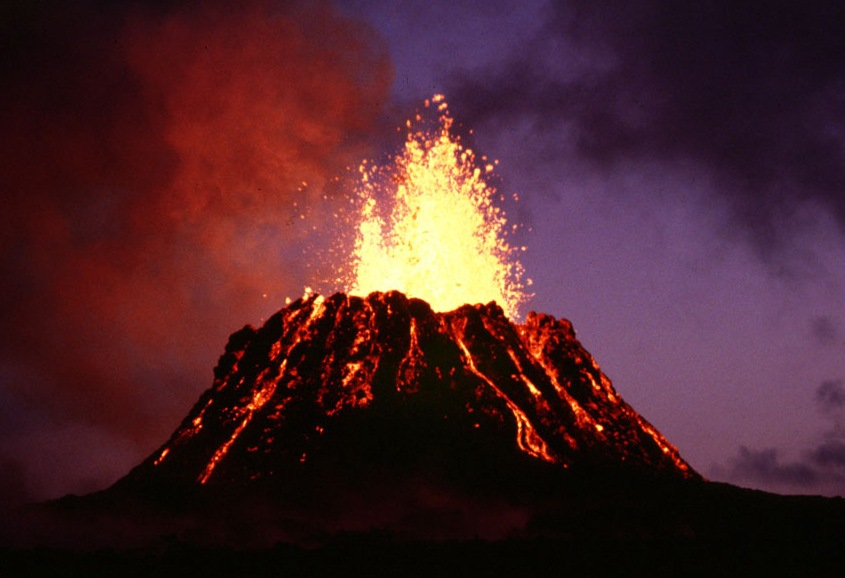
\includegraphics[width=0.55\linewidth]{images/book3/b1-puu-oo-1983.jpg}
\par\smallskip{\small Semburan lava di kerucut Pu\textquoteleft
u~\textquoteleft O\textquoteleft o, di zona celah timur Kilauea, 29 Juni 1983, pada tahun pertama
erupsi yang berlangsung puluhan tahun: lava basal, panas dan encer, terlempar dalam pancaran dan
jatuh kembali di sekitar kawah. Foto: G.~E.~Ulrich, U.S. Geological Survey, domain publik
(Wikimedia Commons).}
\label{fig:b1:hotspots:puu-oo}
\end{omfigure}
% ledger: commons:puu-oo, pp1801:kilauea-rate

\begin{history}[Kerangka tetap untuk lempeng-lempeng]
Pada 1963 John Tuzo Wilson menjelaskan Kepulauan Hawaii, yang semakin tua sepanjang sebuah garis,
dengan sebuah sumber lava yang tertahan di inti lambat sebuah sel konveksi \omterm{def:b1:layered-earth:layers}{mantel}, sementara bagian
atas sel yang lebih cepat membawa dasar laut melintasinya. Pada 1971 dan 1972 W. Jason Morgan
menjadikan sumber itu sebuah plume, selebar sekitar \qty{150}{km}, yang naik dari bagian terbawah
\omterm{def:b1:layered-earth:layers}{mantel} dan karenanya hampir tetap sementara lempeng bergerak di atasnya; eksperimen tangki segera
memperlihatkan bagaimana plume semacam itu tampak. \omterm{def:b1:hotspots:hotspot}{Hotspot} menjadi kerangka tempat lempeng-lempeng
dapat diukur terhadap \omterm{def:b1:layered-earth:layers}{mantel}, bukan hanya terhadap satu sama lain. Setengah abad kemudian kerangka
itu diketahui bergeser, termasuk \omterm{def:b1:hotspots:hotspot}{hotspot} Hawaii di antara yang lain, tetapi cukup lambat sehingga
jejak Pasifik masih memberikan gerak lempeng di atas \omterm{def:b1:layered-earth:layers}{mantel} hingga beberapa derajat dan beberapa
sentimeter setahun, seperti ditunjukkan kecocokan bab ini.
\end{history}
% ledger: hist:plumes, tarduno:emperor

\section{Provinsi beku besar}\label{sec:b1:hotspots:lips}

\begin{definition}[Provinsi beku besar]\label{def:b1:hotspots:lip}
Sebuah \emph{provinsi beku besar}\index{provinsi beku besar} (LIP) adalah akumulasi batuan beku, sebagian besar basal, yang tidak dibuat oleh penyebaran biasa di punggungan, menutupi lebih dari \qty{e5}{km^2}, memuat lebih dari \qty{e5}{km^3}, dan ditempatkan dalam waktu paling lama sekitar 50 juta tahun, sebagian besar dalam denyut-denyut selama 1 hingga 5 juta tahun yang membawa lebih dari tiga perempat volumenya. Di darat LIP sebagian besar berupa basal banjir; di laut, dataran tinggi samudra.
\end{definition}

Sebuah LIP tipikal menutupi sekitar satu juta kilometer persegi dan memuat sekitar satu juta kilometer kubik lava, sebagian besar meletus dalam sekitar satu juta tahun atau kurang. Lavanya ditumpuk dalam aliran yang hampir mendatar, yang dipotong erosi menjadi undakan, \emph{trap} yang memberi nama mereka. Tabel mendaftar yang utama dari 260 juta tahun terakhir.
% ledger: be08:definition, cr03:summary

\begin{omfigure}
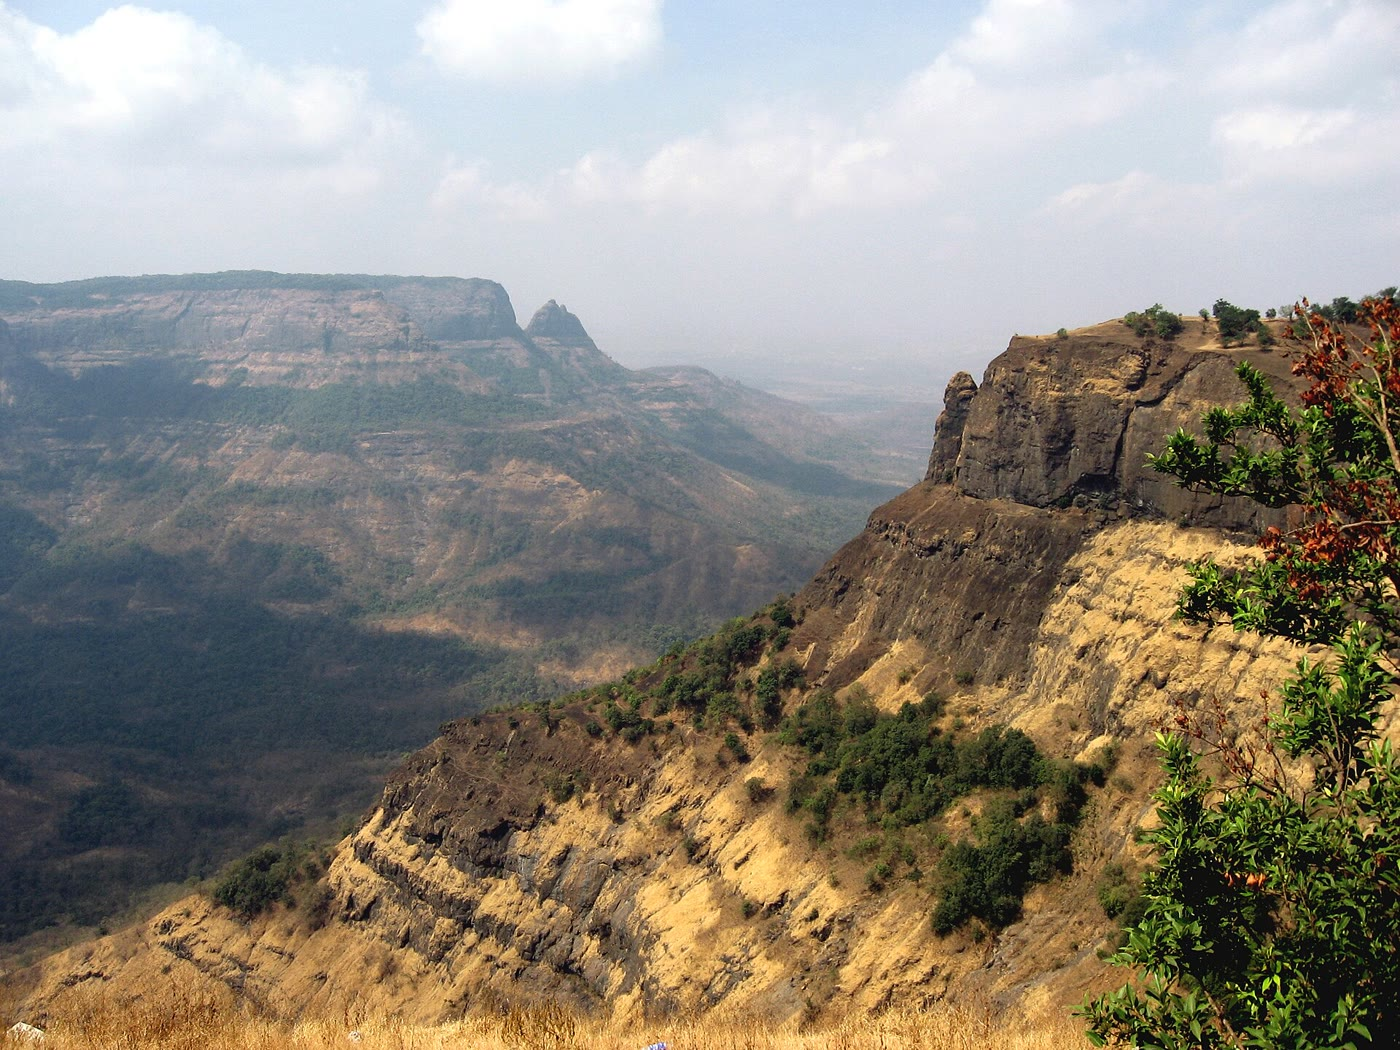
\includegraphics[width=0.55\linewidth]{images/book3/b1-deccan-matheran.jpg}
\par\smallskip{\small Ghats Barat dekat Matheran, India: bukit-bukit berpuncak datar yang terpotong ke dalam tumpukan aliran lava yang hampir mendatar dari Deccan Traps, yang lapisan-lapisannya yang tahan membentuk undakan lereng. Foto: Nicholas (Nichalp), CC BY-SA 2.5 (Wikimedia Commons).}
\label{fig:b1:hotspots:deccan}
\end{omfigure}
% ledger: commons:matheran

\begin{center}
\small
\begin{tabular}{llll}
\hline
provinsi & umur (Ma) & luas (\unit{Mkm^2}) & volume awal (\unit{Mkm^3})\\
\hline
Sungai Columbia & 16 & 0.2 & 0.2\\
Etiopia--Yaman & 30 & 0.7 & 1.2\\
Atlantik Utara & 61 dan 56 & 1.2 & lebih dari 2\\
Deccan & 65.5 & 0.5 (pernah 1.8) & 2 hingga 4\\
Ontong Java & 122 dan 90 & 2 & 44 (seluruh \omterm{def:b1:layered-earth:layers}{kerak})\\
Paraná--Etendeka & 133 & 1.5 (pernah lebih dari 2) & lebih dari 2.3\\
Karoo--Ferrar & 183 & 3.1 & lebih dari 2.5\\
Atlantik Tengah (CAMP) & 201 & pernah hingga 7 & lebih dari 2\\
Trap Siberia & 250 & 0.4 (pernah lebih dari 4) & lebih dari 3\\
Emeishan & 259 & 0.5 (pernah 2 hingga 5) & lebih dari 1\\
\hline
\end{tabular}
\par\smallskip{\small Umur rata-rata; luas seperti hari ini, dan seperti pertama meletus di tempat ada perkiraannya; volume lava seperti pertama meletus, kecuali Dataran Tinggi Ontong Java, yang angkanya menghitung seluruh \omterm{def:b1:layered-earth:layers}{kerak} yang menebal. Data: V.~Courtillot dan P.~Renne (2003).}
\end{center}
% ledger: cr03:table

\noindent Model plume yang digambarkan di \cref{sec:b1:hotspots:plumes} menjelaskan baik ukurannya maupun ketergesaannya: kepala plume selebar ratusan kilometer mencapai dasar \omterm{def:b1:layered-earth:lithosphere}{litosfer}, menurun tekanannya dan meleleh, lalu membanjiri permukaan; kemudian ekornya terus membangun \omterm{def:b1:hotspots:track}{jejak hotspot} biasa. Beberapa provinsi diperkirakan berdiri di ujung tua sebuah jejak yang masih hidup: Deccan Traps dan \omterm{def:b1:hotspots:hotspot}{hotspot} Réunion, Paraná--Etendeka dan Tristan da Cunha, yang dihubungkan oleh Punggungan Walvis, serta basal Columbia River dan Yellowstone.
% ledger: cr03:deccan (Reunion hot spot, plume-head model), be08:ojmh (Parana-Etendeka-Walvis-Tristan), pm90:track (Columbia River basalts)

Deccan Traps di India tengah-barat adalah tumpukan aliran lava setebal sekitar \qty{2500}{m}, yang sekurang-kurangnya \qty{1800}{m} meletus dekat 65.5 juta tahun lalu, dalam waktu jauh kurang dari satu juta tahun; hari ini mereka menutupi sekitar \qty{0.5}{\mega km^2}, mungkin \qty{1.8}{\mega km^2} sebelum erosi. Dataran Tinggi Ontong Java, di Pasifik barat daya, adalah yang terbesar dari semua dataran tinggi samudra: ia menutupi sekitar \qty{2}{\mega km^2}, dan \omterm{def:b1:layered-earth:layers}{keraknya}, sekitar \qty{36}{km} tebalnya, memuat sekitar \qty{44}{\mega km^3} batuan beku. Dataran Tinggi Manihiki dan Hikurangi, kini jauh darinya di seberang dasar samudra yang lebih muda, mungkin terbentuk bersamanya sebagai satu dataran tinggi. Provinsi Magmatik Atlantik Tengah, yang meletus sekitar 201 juta tahun lalu ketika Atlantik mulai terbuka, kini tersebar, sebagai lava, dike dan sill, di atas empat benua: Amerika Utara bagian timur, Amerika Selatan bagian timur laut, Afrika Barat dan Eropa barat daya; ia mungkin pernah menutupi hingga \qty{7}{\mega km^2}.
% ledger: cr03:deccan, cr03:table, cr03:ontong-java, be08:ojmh, cr03:camp


Beberapa provinsi bertepatan waktunya dengan kepunahan massal besar yang digambarkan biologi: Trap Siberia dengan yang terbesar dari semuanya, pada akhir Permian; provinsi Atlantik Tengah dengan akhir Trias; Karoo--Ferrar dengan kepunahan di Jura Awal; Emeishan dengan satu di Permian Tengah; dan Deccan Traps dengan akhir Kapur. Empat kepunahan terbesar dalam 260 juta tahun terakhir masing-masing jatuh, sedekat yang dapat diberikan oleh tanggal-tanggalnya, pada salah satu provinsi ini, dan hubungan sebab-akibat dianggap yang paling mungkin. Mekanisme yang diusulkan bersifat atmosfer: aerosol sulfat yang mendinginkan iklim untuk waktu singkat, karbon dioksida yang menghangatkannya jauh lebih lama, dan samudra yang kekurangan oksigen. Untuk akhir Kapur, letusan Deccan dimulai sebelum tumbukan di Chicxulub dan berlanjut sesudahnya; tinjauan atas catatan batas itu yang disimpulkan pada 2010 menyatakan bahwa tumbukanlah yang memicu kepunahan.
% ledger: cr03:table, cr03:summary, cr03:deccan, schulte:kpg

Tidak semua vulkanisme jauh dari batas lempeng memerlukan plume. Lapangan vulkanik kecil tumbuh di tempat lempeng teregang atau retak, dan rantai tanpa \omterm{def:b1:hotspots:track}{progresi umur} yang bersih mungkin diberi makan dari \omterm{def:b1:layered-earth:layers}{mantel} atas; inilah hipotesis lempeng yang bekerja. Apa yang terjadi pada pulau-pulau samudra setelah \omterm{def:b1:hotspots:hotspot}{hotspot} meninggalkannya, ketika mereka tenggelam, aus dan membentuk terumbu, termasuk dalam volume Tahun ke-2.
% ledger: fn03:plate-hypothesis

\section{Latihan}

\begin{exercise}[$\star$]\label{exo:b1:hotspots:1}
(a) Mauna Kea menjulang \qty{4205}{m} di atas permukaan laut, dan dasar laut jauh dari rantai Hawaii terletak \qty{5274}{m} dalamnya. Berapa tinggi gunung api itu di atas dasar tersebut? Mengapa tinggi sebenarnya dari dasarnya masih lebih besar? (b) Mauna Loa memuat sekitar \qty{74000}{km^3}. Berapa lama waktu yang diperlukan untuk membangunnya dengan pasokan Kilauea saat ini, \qty{0.1}{km^3} setahun, dan dengan laju rata-rata seluruh rantai, \qty{0.025}{km^3} setahun? (c) Erupsi Pu\textquoteleft
u~\textquoteleft O\textquoteleft o mengalirkan sekitar \qty{0.12}{km^3} setahun dari 1983 hingga 2002. Berapa volume itu, dan berapa bagian dari Mauna Loa?
% ledger: pp1801:volumes, pp1801:kilauea-supply, pp1801:chain-volume, pp1801:kilauea-rate; 5274 m from hotspots.py
\end{exercise}

\begin{exercise}[$\star$]\label{exo:b1:hotspots:2}
Sebuah lempeng berputar di atas \omterm{def:b1:hotspots:hotspot}{hotspot-hotspot} dengan \qty{0.92}{\degree\per\Ma}. Ambil $R = \qty{6371}{km}$. (a) Nyatakan $\omega$ dalam radian per juta tahun. (b) Hitung laju, dalam \unit{mm.yr^{-1}}, \omterm{def:b1:hotspots:hotspot}{hotspot} pada \ang{30}, \ang{60}, \ang{90} dan \ang{108.0} dari kutub. (c) Mengapa laju Hawaii, pada \ang{108.0}, lebih kecil daripada pada \ang{90}?
\end{exercise}

\begin{exercise}[$\star$]\label{exo:b1:hotspots:3}
(a) Hitung ketebalan rata-rata Deccan Traps seperti hari ini, \qty{1}{\mega km^3} di atas \qty{0.5}{\mega km^2}, dan provinsi Atlantik Tengah, \qty{2}{\mega km^3} di atas \qty{7}{\mega km^2}. (b) Bandingkan dengan ketebalan penampang Deccan, \qty{2500}{m}. (c) Mengapa ketebalan rata-rata provinsi Atlantik Tengah sedikit mengatakan tentang ketebalan tumpukan lavanya?
% ledger: cr03:table, cr03:deccan, cr03:camp
\end{exercise}

\begin{exercise}[$\star$]\label{exo:b1:hotspots:4}
Batuan plume yang \qty{250}{K} lebih panas daripada \omterm{def:b1:layered-earth:layers}{mantel} di sekitarnya memiliki $\alpha = \qty{3.2e-5}{K^{-1}}$ dan $\rho_m = \qty{3300}{kg.m^{-3}}$. (a) Seberapa jauh ia lebih ringan, dalam \unit{kg.m^{-3}}? (b) Berapa tebal batuan seperti itu, yang tersebar di bawah lempeng, yang akan menopang secara isostatik tonjolan setinggi \qty{690}{m} di bawah laut ($\rho_w = \qty{1000}{kg.m^{-3}}$)?
% ledger: herzberg:tp (200-300 K), parsons:plate-model (alpha)
\end{exercise}

\begin{exercise}[$\star\star$]\label{exo:b1:hotspots:5}
Dua \omterm{def:b1:hotspots:hotspot}{hotspot} terletak di khatulistiwa, A pada \ang{0}\,BT dan B pada \ang{90}\,BT, dan kedua jejak berjalan tepat ke barat (\omterm{def:b1:spherical-astronomy:horizontal}{azimut} \ang{270}). (a) Hitung vektor jejak $\vec t_A$ dan $\vec t_B$. (b) Hitung $\vec t_A\times\vec t_B$. (c) Terapkan aturan tanda \cref{prop:b1:hotspots:two-tracks}: di mana \omterm{def:b1:plate-kinematics:euler-pole}{kutub Euler}? Jelaskan hasilnya tanpa perhitungan. (d) Jika A bergerak pada \qty{50}{mm.yr^{-1}}, berapa $\omega$ dalam derajat per juta tahun?
\end{exercise}

\begin{exercise}[$\star\star$]\label{exo:b1:hotspots:6}
Tiga \omterm{def:b1:hotspots:hotspot}{hotspot} satu lempeng berada pada jarak $x = R\sin\Delta = 3000$, 5000 dan \qty{6000}{km} dari sumbu rotasi dan bergerak dengan 30, 48 dan \qty{57}{mm.yr^{-1}}. (a) Cocokkan $v = \omega x$ dengan kuadrat terkecil dan berikan $\omega$ dalam radian dan dalam derajat per juta tahun. (b) Hitung residunya. (c) Mengapa garis itu harus melalui titik asal?
\end{exercise}

\begin{exercise}[$\star\star$]\label{exo:b1:hotspots:7}
Sebuah tonjolan dengan penampang \qty{3e8}{m^2} mengelilingi \omterm{def:b1:hotspots:track}{jejak hotspot} di atas lempeng yang bergerak dengan \qty{50}{mm.yr^{-1}}. Ambil $\rho_m - \rho_w = \qty{2300}{kg.m^{-3}}$, $c_p = \qty{910}{J.kg^{-1}.K^{-1}}$ dan $\alpha = \qty{3.2e-5}{K^{-1}}$. (a) Hitung fluks daya apungnya dan fluks panasnya. (b) Bandingkan dengan Hawaii, \qty{3240}{kg.s^{-1}}. (c) Dua \omterm{def:b1:hotspots:hotspot}{hotspot} memiliki tonjolan yang sama; satu berada di bawah lempeng yang bergerak dua kali lebih cepat. Plume mana yang lebih kuat?
\end{exercise}

\begin{exercise}[$\star\star$]\label{exo:b1:hotspots:8}
Sepanjang jejak Yellowstone, letusan kaldera dimulai di medan vulkanik McDermitt 16.1 juta tahun lalu dan di medan Picabo, sekitar \qty{350}{km} ke timur laut, 10.3 juta tahun lalu; sejak itu mereka bergerak dengan $\qty[uncertainty-mode=separate]{2.9 \pm 0.5}{cm}$ setahun ke arah U\,\ang{54}\,T. (a) Pada laju rata-rata berapa vulkanisme bermigrasi dari McDermitt ke Picabo? (b) Bandingkan kedua laju dengan laju lempeng di atas \omterm{def:b1:hotspots:hotspot}{hotspot}, \qty[uncertainty-mode=separate]{26 \pm 5}{mm.yr^{-1}} ke arah \ang{235}. (c) Apakah arah jejak muda itu seperti yang diharapkan? (d) Bagian tua dari jejak itu terletak di wilayah yang teregang ketika vulkanisme melewatinya. Bagaimana hal ini dapat menjelaskan selisihnya?
% ledger: pm90:track, data:b3-hotspots
\end{exercise}

\begin{exercise}[$\star\star$]\label{exo:b1:hotspots:9}
Plume Hawaii membawa sekitar \qty{9.2e10}{W} panas berlebih. (a) Jika seluruhnya keluar melalui dasar laut \qty{1000}{km} kali \qty{1000}{km} yang terdekat dengan \omterm{def:b1:hotspots:hotspot}{hotspot}, seberapa besar \omterm{def:b1:heat-budget:heat-flow}{aliran panas} di sana akan naik? (b) Bandingkan dengan kelebihan yang teramati, paling tinggi 5 hingga \qty{10}{mW.m^{-2}}. (c) Berapa lama panas memerlukan waktu untuk berdifusi melalui lempeng setebal \qty{100}{km} ($\kappa = \qty{e-6}{m^2.s^{-1}}$)? Berapa lama lempeng memerlukan waktu untuk menyeberangi \qty{1000}{km} pada \qty{92}{mm.yr^{-1}}? Simpulkan.
% ledger: vh89:swell-heat
\end{exercise}

\begin{exercise}[$\star\star\star$]\label{exo:b1:hotspots:10}
Trap Deccan memuat sekitar \qty{e6}{km^3} lava. Anggap ia berasal dari kepala plume berbentuk bola yang sepersepuluhnya meleleh. (a) Berapa volume dan jari-jari kepala itu? (b) Setelah diratakan di bawah \omterm{def:b1:layered-earth:lithosphere}{litosfer} menjadi piringan setebal \qty{100}{km}, berapa diameter kepala itu? Bandingkan luasnya dengan luas yang pernah ditutupi Trap, \qty{1.8}{\mega km^2}. (c) Jika lava meletus dalam satu juta tahun, bandingkan lajunya dengan pasokan Kilauea saat ini, \qty{0.1}{km^3} setahun. (d) Mengapa kepala plume harus besar, sementara ekor yang mengikutinya sempit?
% ledger: cr03:table, pp1801:kilauea-supply
\end{exercise}

\begin{exercise}[$\star\star\star$]\label{exo:b1:hotspots:11}
Antara 81 dan 47 juta tahun lalu \omterm{def:b1:hotspots:hotspot}{hotspot} Hawaii bergerak ke selatan dengan lebih dari \qty{40}{mm.yr^{-1}}. (a) Dengan \qty{40}{mm.yr^{-1}}, seberapa jauh ia bergerak? (b) Anggap lempeng bergerak selama itu dengan \qty{80}{mm.yr^{-1}} ke arah \ang{340} di atas \omterm{def:b1:layered-earth:layers}{mantel} dalam. Dengan $x$ ke timur dan $y$ ke utara, hitung kecepatan lempeng relatif terhadap \omterm{def:b1:hotspots:hotspot}{hotspot} yang hanyut, lajunya dan \omterm{def:b1:spherical-astronomy:horizontal}{azimutnya}. (c) Dengan berapa persen, dan dengan berapa derajat, jejak yang dibangun saat itu akan salah menggambarkan gerak lempeng di atas \omterm{def:b1:layered-earth:layers}{mantel} dalam?
% ledger: tarduno:emperor
\end{exercise}

\begin{exercise}[$\star\star\star$]\label{exo:b1:hotspots:12}
(a) Sebuah basal banjir sebesar \qty{e6}{km^3} mendingin dari sekitar \qty{1300}{\celsius} hingga suhu permukaan. Dengan kapasitas panas \qty{3}{MJ.m^{-3}.K^{-1}}, berapa panas yang dilepaskannya (abaikan panas laten kristalisasi)? (b) Tersebar dalam satu juta tahun, berapa daya itu? Bandingkan dengan plume Hawaii, \qty{9.2e10}{W}, dan dengan \qty{47}{TW} seluruh Bumi. (c) Kepala plume juga memanaskan dasar \omterm{def:b1:layered-earth:lithosphere}{litosfer} tanpa melelehkan seluruhnya. Apakah daya pada (b) merupakan batas atas atau batas bawah panas yang dibawa kepala itu?
% ledger: delaney86:properties (Book 2 row, 2-3 MJ/m3/K), dd10:total; 1300 degC is an exercise value
\end{exercise}

\section{Masalah: penunjuk kecepatan Lempeng Pasifik}

\begin{problem}[{Soal akhir pekan --- penunjuk kecepatan Lempeng Pasifik: kutub Euler dari dua jejak hotspot, lajunya dari pengukuran ketiga, uji pada hotspot lain, dan daya apung serta pasokan plume Hawaii}]
\label{pb:b1:hotspots:1}
% values: calc/ch15.py; ledger: data:b3-hotspots, data:etopo1, pp1801:kilauea-supply, pp1801:volumes,
% pp1801:chain-volume, delaney86:properties, parsons:plate-model, dd10:total, data:pb2002 (ridge_budget.py), cd87:rate
Morgan dan Morgan mencantumkan \omterm{def:b1:hotspots:hotspot}{hotspot} Hawaii pada \ang{19.0}\,LU, \ang{155.2}\,BB, dengan jejak ke arah $\ang{304}\pm\ang{3}$ dan laju \qty[uncertainty-mode=separate]{92 \pm 3}{mm.yr^{-1}}, dan \omterm{def:b1:hotspots:hotspot}{hotspot} Louisville pada \ang{53.6}\,LS, \ang{140.6}\,BB, dengan jejak ke arah $\ang{316}\pm\ang{5}$ dan laju \qty[uncertainty-mode=separate]{67 \pm 5}{mm.yr^{-1}}. Gunakan sumbu dan vektor $\vec e$, $\vec n$, $\vec t$ dari \cref{sec:b1:hotspots:tracks}, dengan $R = \qty{6371}{km}$. Berikan komponen hingga empat desimal.

\medskip
\noindent\textbf{Bagian I --- Kutub dari dua jejak.}
\begin{enumerate}
  \item Hitung $\vec r$, $\vec e$ dan $\vec n$ di Hawaii, lalu vektor jejak $\vec t_H$.
  \item Lakukan hal yang sama di Louisville: $\vec r_L$, $\vec e$, $\vec n$ dan $\vec t_L$.
  \item Periksa bahwa $\vec t_H$ adalah vektor satuan yang tegak lurus terhadap $\vec r_H$.
  \item Hitung $\vec t_H\times\vec t_L$ dan panjangnya. Berapa sudut yang dibentuk kedua vektor jejak?
  \item Normalkan hasil kali silang dan terapkan aturan tanda \cref{prop:b1:hotspots:two-tracks}.
  \item Berikan \omterm{def:b1:spherical-astronomy:geographic}{lintang} dan \omterm{def:b1:spherical-astronomy:geographic}{bujur} \omterm{def:b1:plate-kinematics:euler-pole}{kutub Euler} Lempeng Pasifik terhadap \omterm{def:b1:hotspots:hotspot}{hotspot}.
\end{enumerate}

\medskip
\noindent\textbf{Bagian II --- Laju.}
\begin{enumerate}[resume]
  \item Hitung jarak sudut $\Delta_H$ dan $\Delta_L$ dari kutub ke kedua \omterm{def:b1:hotspots:hotspot}{hotspot}.
  \item Hitung $(\vec p\times\vec r_L)\cdot\vec t_L$. Jelaskan mengapa ia sama dengan $\sin\Delta_L$, dan apa tandanya mengatakan tentang gerak di Louisville.
  \item Dari laju di Louisville, hitung $\omega$ dalam radian dan dalam derajat per juta tahun.
  \item Berapa lama Lempeng Pasifik memerlukan waktu untuk membuat satu putaran penuh terhadap kutub ini?
  \item Kutub kuadrat terkecil dari lima belas jejak Pasifik terletak pada \ang{63.78}\,LS, \ang{112.48}\,BT, dengan \qty{0.92}{\degree\per\Ma}. Hitung sudut antara kedua kutub dan bandingkan kedua laju.
\end{enumerate}

\medskip
\noindent\textbf{Bagian III --- Uji pada tiga hotspot lain.} Morgan dan Morgan memberikan \omterm{def:b1:hotspots:hotspot}{hotspot} Society (\ang{18.2}\,LS, \ang{148.4}\,BB)
\qty[uncertainty-mode=separate]{109 \pm 10}{mm.yr^{-1}}, Pitcairn
(\ang{25.4}\,LS, \ang{129.3}\,BB)
\qty[uncertainty-mode=separate]{90 \pm 15}{mm.yr^{-1}} dan Cobb
(\ang{46.0}\,LU, \ang{130.1}\,BB)
\qty[uncertainty-mode=separate]{43 \pm 3}{mm.yr^{-1}}.
\begin{enumerate}[resume]
  \item Hitung jarak sudut dari kutub pada soal 6 ke masing-masing dari ketiga \omterm{def:b1:hotspots:hotspot}{hotspot} itu.
  \item Prediksikan ketiga laju dengan laju pada soal 9.
  \item Prediksi mana yang sesuai dengan laju yang terukur dalam ketidakpastiannya, dan mana yang tidak?
  \item Dua jejak dengan arah berbeda selalu memberi sebuah kutub. Mengapa dua jejak yang hampir sejajar merupakan pilihan yang buruk?
\end{enumerate}

\medskip
\noindent\textbf{Bagian IV --- Plume dan penunjuk kecepatan.} Tonjolan Hawaii memiliki penampang \qty{4.83e8}{m^2}. Ambil $\rho_m - \rho_w = \qty{2300}{kg.m^{-3}}$, $c_p = \qty{910}{J.kg^{-1}.K^{-1}}$ dan $\alpha = \qty{3.2e-5}{K^{-1}}$.
\begin{enumerate}[resume]
  \item Ubah \qty{92}{mm.yr^{-1}} ke \unit{m.s^{-1}} dan hitung fluks daya apung plume Hawaii.
  \item Hitung panas berlebih yang dibawanya, dan bandingkan dengan \qty{47}{TW} yang keluar dari Bumi.
  \item Punggungan membuat sekitar \qty{21}{km^3} \omterm{def:b1:layered-earth:layers}{kerak} setiap tahun sepanjang sekitar \qty{67000}{km}. Berapa panjang punggungan yang membuat \omterm{def:b1:layered-earth:layers}{kerak} sebanyak yang dipasok ke Kilauea, \qty{0.1}{km^3} setahun?
  \item Dengan laju itu, berapa lama Mauna Loa, sekitar \qty{74000}{km^3}, memerlukan waktu untuk tumbuh?
  \item \omterm{def:b1:hotspots:hotspot}{Hotspot} membangun sekitar \qty{2e6}{km^3} rantai dalam 81 juta tahun. Hitung keluaran rata-ratanya dan bandingkan dengan pasokan Kilauea hari ini.
  \item Dengan kutub dan laju dari Bagian I dan II, hitung laju yang diprediksi jejak Louisville untuk Lempeng Pasifik di atas \omterm{def:b1:hotspots:hotspot}{hotspot} Hawaii.
  \item Bandingkan dengan \qty[uncertainty-mode=separate]{92 \pm 3}{mm.yr^{-1}} yang terukur: sebesar berapa, dan dengan berapa simpangan baku, keduanya berbeda?
  \item Dari umur gunung-gunung api Hawaii, Buku 2 menemukan \qty{9.1}{cm} setahun, dan penulis umur-umur itu, dengan mencocokkan seluruh rantai, \qty{8.6}{cm} setahun. Bandingkan rata-rata ini selama puluhan juta tahun dengan kedua laju \omterm{def:b1:hotspots:hotspot}{hotspot}.
  \item Hingga satu desimal, dalam sentimeter setahun, laju apa yang diberikan jejak Louisville untuk Lempeng Pasifik di atas \omterm{def:b1:hotspots:hotspot}{hotspot} Hawaii?
\end{enumerate}
\end{problem}
